In practise arbitrage is the process of buying something at price $x$ and instantly selling it a price $y$ where $x<y$. Arbitrage is risk-free, if we make some assumptions; since we perform it instantly we can gaurentee that $x<y$, and we do not take into account the inherit volunerabilities of bugs in smart contracts.

When determining the arbitrage opportunity it is a bit more complicated since prices of assets are not static but determined by market behaviours. We can see the prices of assets at the different decentralized exchanges, as we defined in the background section there are two main forms of exchanges, the simpler one being the limit order book. When performing arb on LOB DEX's we check if there is some asset (ABC) that has an overlapping price, an example of this can be seen in figure \ref{fig:ArbLOB} 

\begin{figure}
\centering
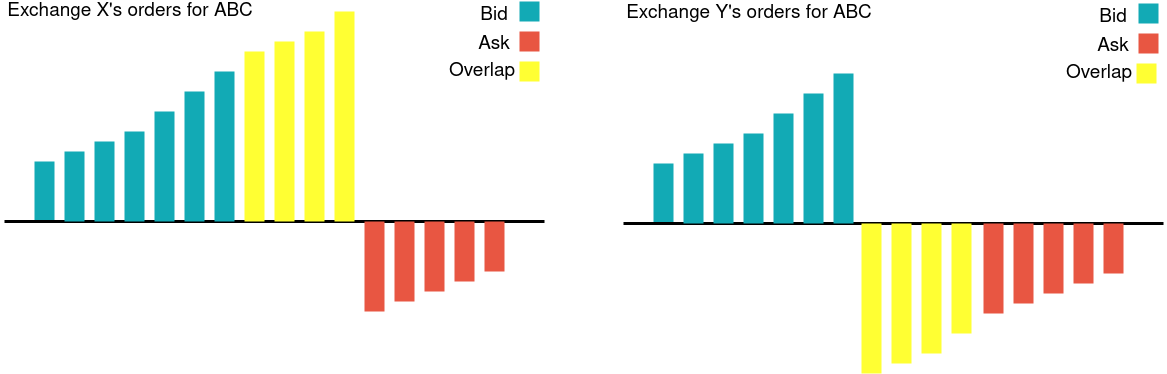
\includegraphics[width=0.7\textwidth]{assests/Flash-loans-Arbitrage-Overlap-1}
\caption{Arbitrage on LOB DEX}
\label{fig:ArbLOB}
\end{figure}